\chapter{Experimentos} \label{cap:cap5}

Foram feitos experimentos como parte do projeto aprovado no comitê de ética do Hospital Universitário Antônio Pedro associado a faculdade de medicina da Universidade Federal Fluminense. Este projeto foi registrado na Plataforma Brasil do ministério da saúde sob o número 23637019.5.0000.5243. A descrição destes experimentos e discussão dos resultados obtidos foram publicados em conferência da área \cite{Melo2021}.

Os experimentos foram apresentados a doze voluntários que fizeram uso do equipamento háptico, todos estes voluntários foram estudantes de ciência da computação com idades variando entre 18 e 44 anos sendo que onze homens e uma mulher. Todos os voluntários assinaram o termo de consentimento de participação nesta pesquisa. Todos receberam uma breve explicação (cinco minutos) a respeito do procedimento de uso do equipamento háptico no experimento e tiveram mais outros cinco minutos de tempo para usar um aplicativo de exemplo para adquirir conhecimento sobre como interagir num ambiente com este tipo de dispositivo visando nivelar o conhecimento.

Nos experimentos foi utilizado o dispositivo háptico \textit{Geomagic Touch®}. Para este uso foi necessária a instalação do \texit{OpenHaptics Touch Device Driver} que está disponível no endereço eletrônico da empresa responsável pela produção e comercialização deste dispositivo háptico \cite{3DSystemsTouch2018}. Também foi utilizado um \textit{plugin} \cite{Poyade2014} para programação das interações com o háptico utilizando o motor de jogo da \textit{Unity} \cite{UnityTechnologies2020} que é uma ferramenta muito utilizada para desenvolvimento de videogames e simulações com e sem \acrshort{RV} para diversas plataformas.
Este \textit{plugin} possibilita a interação do usuário com os objetos no ambiente virtual  de quatro modos distintos. Para este experimento utilizamos o modo \textit{Puncture} (modo de punção) pelo requisito do experimento em simular uma agulha sendo inserida através de camadas representativas de tecidos.

\textit{OpenHaptics driver} possui um conjunto de propriedades que representam como qualquer objeto 3D (camada, superfície, etc) tocável do ambiente virtual desenvolvido reage a cada interação com o dispositivo háptico. As propriedade mais relevantes no contexto do modo de punção são \textit{Stiffness}, \textit{Pop Through}, \textit{Static Friction}, e \textit{Dynamic Friction}. Todas elas tem como domínio um número real e aceita valores entre zero e um. 

\texit{Stiffness} representa o nível de dureza do objeto: zero (0) representa um objeto mole e um (1) o objeto mais duro possível \cite{3DSystemsTouch2018}. Neste ponto é importante ressaltar que a quantidade de força máxima suportada depende das especificações do dispositivo háptico usado, dispositivos mais simples e de custo mais baixo comumente suportam intensidades de forças menores se comparadas a dispositivos mais complexos e com custos mais altos. \textit{Pop Through} controla o nível de força necessária para perfurar um objeto: zero indica que o objeto não pode ser perfurado e um que o máximo de força é necessário para perfurar o objeto \cite{3DSystemsTouch2018}. \textit{Punctured Static Friction} configura a dificuldade de se mover dentro de um objeto perfurado a partir de uma posição estática. O limite inferior (zero) representa um movimento sem atrito e o limite superior (um) representa a quantidade maior de atrito suportada pelo dispositivo \cite{3DSystemsTouch2018}. \textit{Punctured Dynamic Friction} controla a dificuldade de se mover dentro de um objeto depois q o movimento já foi iniciado \cite{3DSystemsTouch2018}. Da mesma forma que no caso estático o zero representa um movimento sem atrito e um o máximo de atrito suportado. Essas propriedades podem ser usadas para configurar o comportamento de cada camada de forma que o usuário tenha um experiência tátil de interação virtual que simule o procedimento real. As propriedades \textit{Stiffness} e \textit{Pop Through} precisam ser configuradas pra se determinar a força necessária por parte do usuário para perfurar cada objeto enquanto para determinar a força necessária para movimentação de uma agulha dentro de um objeto as propriedade a serem configuradas são \textit{Punctured Static Friction} e \textit{Punctured Dynamic Friction}.

Dois experimentos foram construídos para simular as diferentes sensações que os anestesistas experimentam enquanto executam punções lombares. Nestes experimentos os objetos 3D usados para simular as camadas do corpo foram simplificados e representados como hexaedros. Essa abordagem foi utilizada por que o objetivo destes experimentos não era a avaliação estética. Foi removido o modelo 3D já desenvolvido para o simulador e foram utilizados modelos simplificados que não desviassem a atenção dos usuários da avaliação em termos das sensações de perfuração e penetração do objeto 3D que representava a agulha em relação aos objetos que representavam as camadas.
As imagens dos detalhes dos objetos 3D dos dois experimentos podem ser visualizados na Figura \ref{fig:objectsExperiments}. As setas de diferentes tamanhos no eixo Z ilustram as diferenças nos objetos 3D de cada experimento. A primeira camada (mais externa) é um cubo, e as demais camadas tem profundidades menores mas todas tem a mesma largura (eixo X) e altura (eixo Y), como pode ser visto na Figura \ref{fig:objectsExperiments}.

\begin{figure}[ht!]
    \centering
        \begin{tabular}{cc}
        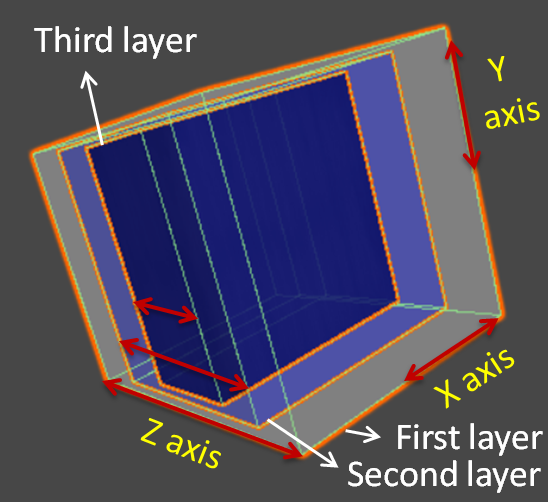
\includegraphics[width=0.3\linewidth]{capitulos/figuras/First.Experiment - axis.PNG} & 
        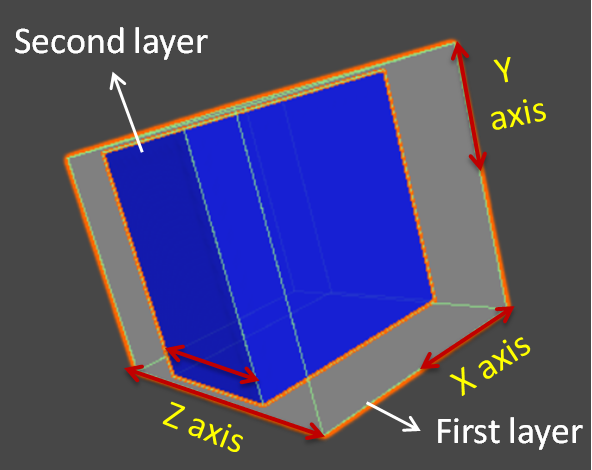
\includegraphics[width=0.35\linewidth]{capitulos/figuras/Second.Experiment - axis.PNG} 
        \\
        (a) & (b)
        \end{tabular}
    \caption{Os objetos 3D representam as camadas de cada experimento: (a) Primeiro experimento (b) Segundo experimento.}
    \label{fig:objectsExperiments}
\end{figure}

O tamanho da agulha é 65 milímetros (mm). Para os dois experimentos foi incluída uma deformação na interface de cada camada com o aumento da força antes da perfuração. Essa deformação é uma função da força necessária para perfurar cada camada. Foi usado um valor máximo de deformação de cinquenta vezes o valor da propriedade \textit{Pop through} em cada camada. O deslocamento desta deformação máxima é medido em milímetros. Logo após ser perfurado o tecido reassume a posição original (sem deformação). 

A Tabela \ref{tab:propHapticoPrimeiroExperimento} descreve os valores configurados nas propriedades de cada camada do primeiro experimento. A deformação máxima para a primeira camada é de is 2,5 mm, que corresponde a cinquenta vezes o 0,05 (\textit{Pop Through} da primeira camada). A Figura \ref{fig:forcaDeslocamentoExperimento1} apresenta um gráfico da aplicação da força (vertical axis) com o deslocamento da agulha representado no eixo horizontal para o experimento 1. As setas nesta imagem indicam a extensão da deformação de cada camada, começando na esquerda quando a agulha começa a tocar a camada e termina na direita quando a camada é perfurada. O espaço entre as setas da Figura \ref{fig:forcaDeslocamentoExperimento1} representa quando a agulha está em movimento dentro das camadas. As menores variações no eixo horizontal são observadas sob a área das setas por conta da necessidade do aumento de força para se perfurar a camada. As diferenças mais significativas no eixo de deslocamento podem ser observados a direita das setas, marcados com retângulos, que representa o aumento da velocidade de deslocamento da agulha imediatamente após a perfuração da camada.

\begin{table}[!ht]
\begin{center}
\caption{Configurações do háptico usadas no primeiro experimento.}
\label{tab:propHapticoPrimeiroExperimento}
\begin{tabular}{|l|lll|}
\hline
\multicolumn{1}{|c|}{\multirow{2}{*}{Propriedade}} & \multicolumn{3}{c|}{Camada}  \\ \cline{2-4} 
\multicolumn{1}{|c|}{} & \multicolumn{1}{c|}{1} & \multicolumn{1}{c|}
{
\begin{tabular}[c]{@{}c@{}}2\end{tabular}} & \multicolumn{1}{c|}{\begin{tabular}[c]{@{}c@{}}3\end{tabular}}  \\ 
\hline\hline
\textit{Stiffness} & \multicolumn{1}{l|}{0,75} & \multicolumn{1}{l|}{0,75} & \multicolumn{1}{l|}{0,75} \\ 
\textit{Pop Through} & \multicolumn{1}{l|}{0,05} & \multicolumn{1}{l|}{0,15} & \multicolumn{1}{l|}{0,10}  \\ 
\textit{Punctured Static Friction} & \multicolumn{1}{l|}{0,20} & \multicolumn{1}{l|}{0,30} & \multicolumn{1}{l|}{0,30}  \\ 
\textit{Punctured Dynamic Friction} & \multicolumn{1}{l|}{0,30} & \multicolumn{1}{l|}{0,30} & \multicolumn{1}{l|}{0,10}  \\ 
\hline
\end{tabular}
\end{center}
\end{table}

O segundo experimento tem duas camadas e sua configuração está descrita na Tabela \ref{tab:propHapticoSegundoExperimento}. A curva de força versus deslocamento da agulha desse experimento está ilustrada na Figura \ref{fig:forcaDeslocamentoExperimento2} e aqui se aplicam as mesmas considerações feitas em relação as marcações de setas e retângulos discutidas em relação a Figura \ref{fig:forcaDeslocamentoExperimento1}.

The starting point (0 mm) is the interface of the first layer in each experiment. This point was chosen as a reference to measure the displacement to reach each of the other layers. The direction of this measure is orthogonal to the user touched surface. The second layer on experiment one is at 25 mm and the third at 50 mm. The second layer of the second experiment is at 35mm of the starting point.

\begin{figure}[ht!]
    \centering
    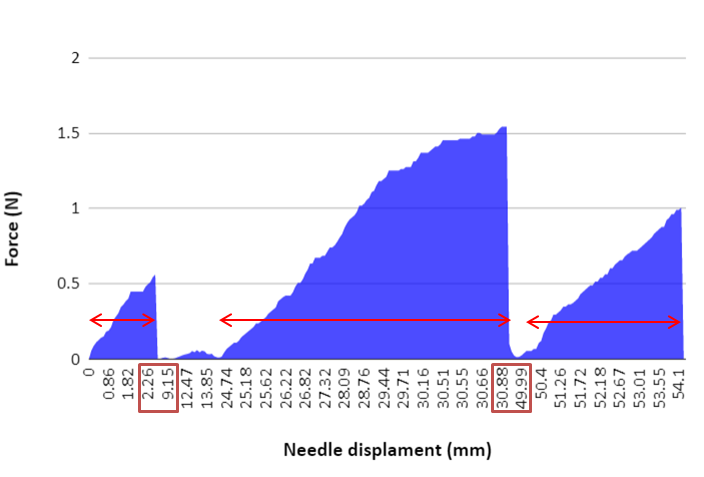
\includegraphics[width=0.8\linewidth]{capitulos/figuras/Experiment 1 - Force x Needle displacement - marked.PNG} 
    \caption{Relação entre força e o deslocamento da agulha da média de dez simulações no experimento 1.}
    \label{fig:forcaDeslocamentoExperimento1}
\end{figure}

\begin{table}[!ht]
\begin{center}
\caption{Configurações do háptico usadas no segundo experimento.}
\label{tab:propHapticoSegundoExperimento}
\begin{tabular}{|l|ll|}
\hline
\multicolumn{1}{|c|}{\multirow{2}{*}{Propriedade}} & \multicolumn{2}{c|}{Camada}  \\ \cline{2-3} 
\multicolumn{1}{|c|}{} & \multicolumn{1}{c|}{1}
{
 \multicolumn{1}{c|}{\begin{tabular}[c]{@{}c@{}}2\end{tabular}}}  \\ 
\hline\hline
\textit{Stiffness} & \multicolumn{1}{l|}{0,75} & \multicolumn{1}{l|}{0,20}  \\ 
\textit{Pop Through} & \multicolumn{1}{l|}{0,05} & \multicolumn{1}{l|}{0,15}  \\ 
\textit{Punctured Static Friction} & \multicolumn{1}{l|}{0,90} & \multicolumn{1}{l|}{0,10}  \\ 
\textit{Punctured Dynamic Friction} & \multicolumn{1}{l|}{0,20} & \multicolumn{1}{l|}{0,10}   \\ 
\hline
\end{tabular}
\end{center}
\end{table}

\begin{figure}[ht!]
    \centering
    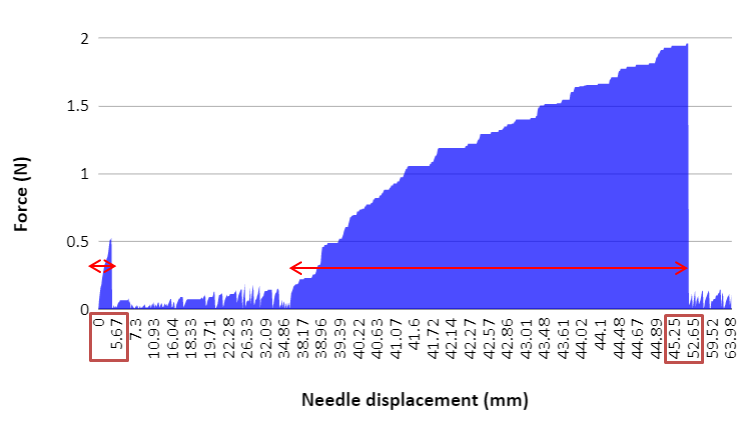
\includegraphics[width=0.8\linewidth]{capitulos/figuras/Experiment 2 - Force x Needle displacement - marked.PNG} 
    \caption{Relação entre força e o deslocamento da agulha da média de dez simulações no experimento 2.}
    \label{fig:forcaDeslocamentoExperimento2}
\end{figure}